\documentclass{article}
\usepackage{array}
\usepackage{graphicx}
\usepackage{fullpage}
\usepackage[svgnames]{xcolor}
\usepackage{color}
\usepackage{fourier}

\newcommand*{\rotrt}[1]{\rotatebox{90}{#1}} % Command to rotate right 90 degrees
\newcommand*{\rotlft}[1]{\rotatebox{-90}{#1}} % Command to rotate left 90 degrees

\newcommand*{\titleBC}{\begingroup % Create the command for including the title page in the document
\centering % Center all text

\def\CP{\textit{\Huge Man JAVANAISE}} % Title

\settowidth{\unitlength}{\CP} % Set the width of the curly brackets to the width of the title
\textcolor{FireBrick}{\CP} \\[\baselineskip] % Print title
{\color{Grey}\Large Distributed object cache management} \\ % Tagline or further description
\endgroup}

\definecolor{lg}{rgb}{0.9,0.9,0.9}

\let\oldv\verbatim
\let\oldendv\endverbatim

\def\verbatim{\setbox0\vbox\bgroup\oldv}
\def\endverbatim{\oldendv\egroup\fboxsep0pt \colorbox[gray]{0.9}{\usebox0}\par}

%%%% Le Document %%%%

\begin{document}

\begin{table}[h]
    \begin{center}
    \begin{tabular}{ >{\centering\arraybackslash}m{1.5in} >{\arraybackslash}m{4in} }

    \vspace{5mm} 
\includegraphics[width=2cm]{logo.jpg} & \vspace{9mm} This \textit{JAVANAISE} librairy was realized as part of the \textit{JAVANAISE Project} for the course of \textit{Advanced Distributed Programming} in \textit{M2PGI}.

The authors are \textbf{Johan GIRARD} and \textbf{Pierre ODIN}.

  \end{tabular}

  \label{tabular:UKJPNdata}
  \end{center}
\end{table}

\hrule\hrule

\vspace{1.5cm}

\titleBC

\vspace{1cm}

\section{Add JAVANAISE in a Project}

To use JAVANAISE, add the librairy and several elements to the Project :
\begin{itemize}
\item Add \texttt{JAVANAISE.jar} to the \textit{Build Path} of the Project.
\item Create a \texttt{save/} directory at the root of the Project.
\item Create a \texttt{java.policy} file at the root of the Project with the following code :
\end{itemize}

\noindent
\begin{verbatim}
    grant{
      permission java.security.AllPermission "", "";
    };
\end{verbatim}

\section{Run the coordinator}

Next, create a class named \texttt{RunCoordinator}. This class is used to start and to configure the coordinator : \\

\noindent
\begin{verbatim}
    import jvn.JvnCoordImpl;

    public class RunCoordinator {
        public static void main(String[] args) {
            JvnCoordImpl.start(false);
        }
    }
\end{verbatim}
\vspace{0.3cm}

\noindent The \texttt{start(...)} method takes a boolean in argument :

\begin{itemize}
\item \texttt{TRUE} $\rightarrow$ The coordinator will restore his old tables (list of objects, servers, locks, ...) when starting.
\item \texttt{FALSE} $\rightarrow$ The coordinator will reset all his tables when starting.
\end{itemize}

\section{Create an Object}

The creation of an object requires 3 steps. Note that the number of different objects created is not limited.

\subsection{Interface}

Start by create an \texttt{Interface} extanding \texttt{JvnTransactionObject}. This Interface contains the definition of all the methods of the object. Each of these methods has to be annotate with \texttt{@JvnWriteMethod} if it's a method which can change the state of the object or with \texttt{@JvnReadMethod} in the other case. \\

\noindent
\begin{verbatim}
    import jvn.JvnTransactionObject;
    import jvn.annots.JvnReadMethod;
    import jvn.annots.JvnWriteMethod;

    public interface IMyObject extends JvnTransactionObject {
	
        @JvnWriteMethod
        public void write(String text);
	
        @JvnReadMethod
        public String read() ;
	
    }
\end{verbatim}

\subsection{Class}

Create a class extanding \texttt{JvnTransactionObjectAbstract} and implementing the previous interface. This class provides the implementation of all the methods of the object. \\

\noindent
\begin{verbatim}
    import jvn.JvnTransactionObjectAbstract; 

    public class MyObject extends JvnTransactionObjectAbstract implements IMyObject { 
	
        ...
        
        public MyObject(){}

        ...
	 
    }
\end{verbatim}

\subsection{Instanciation}

Finally, instanciate the object with the following code : \\

\noindent
\begin{verbatim}
    IMyObject o = (IMyObject) JvnObjectProxy.instanceJvn(new MyObject(), "MYOBJECT");
\end{verbatim}
\vspace{0.3cm}

\noindent The second argument of the \texttt{instanceJvn(...)} method is the id of the object on the coordinator.

\section{Use an Object in a client application}

After the instanciation, the object is ready to be used. Every methods defined on the interface can be called. \\

\noindent
\begin{verbatim}
    o.read();
    o.write("Hello");
    o.read();
    o.write("Bye");
\end{verbatim}

\section{Exit the application}

At the end of the execution of the application, the coordinator needs to be notify in order to remove the server from his tables. Use the following instruction before ending the execution : \\

\noindent
\begin{verbatim}
    JvnServerImpl.jvnGetServer().jvnTerminate();
\end{verbatim}

\section{Simplified diagram of how it works}

The following diagram shows how the caches and the coordinator are used.

\begin{center}
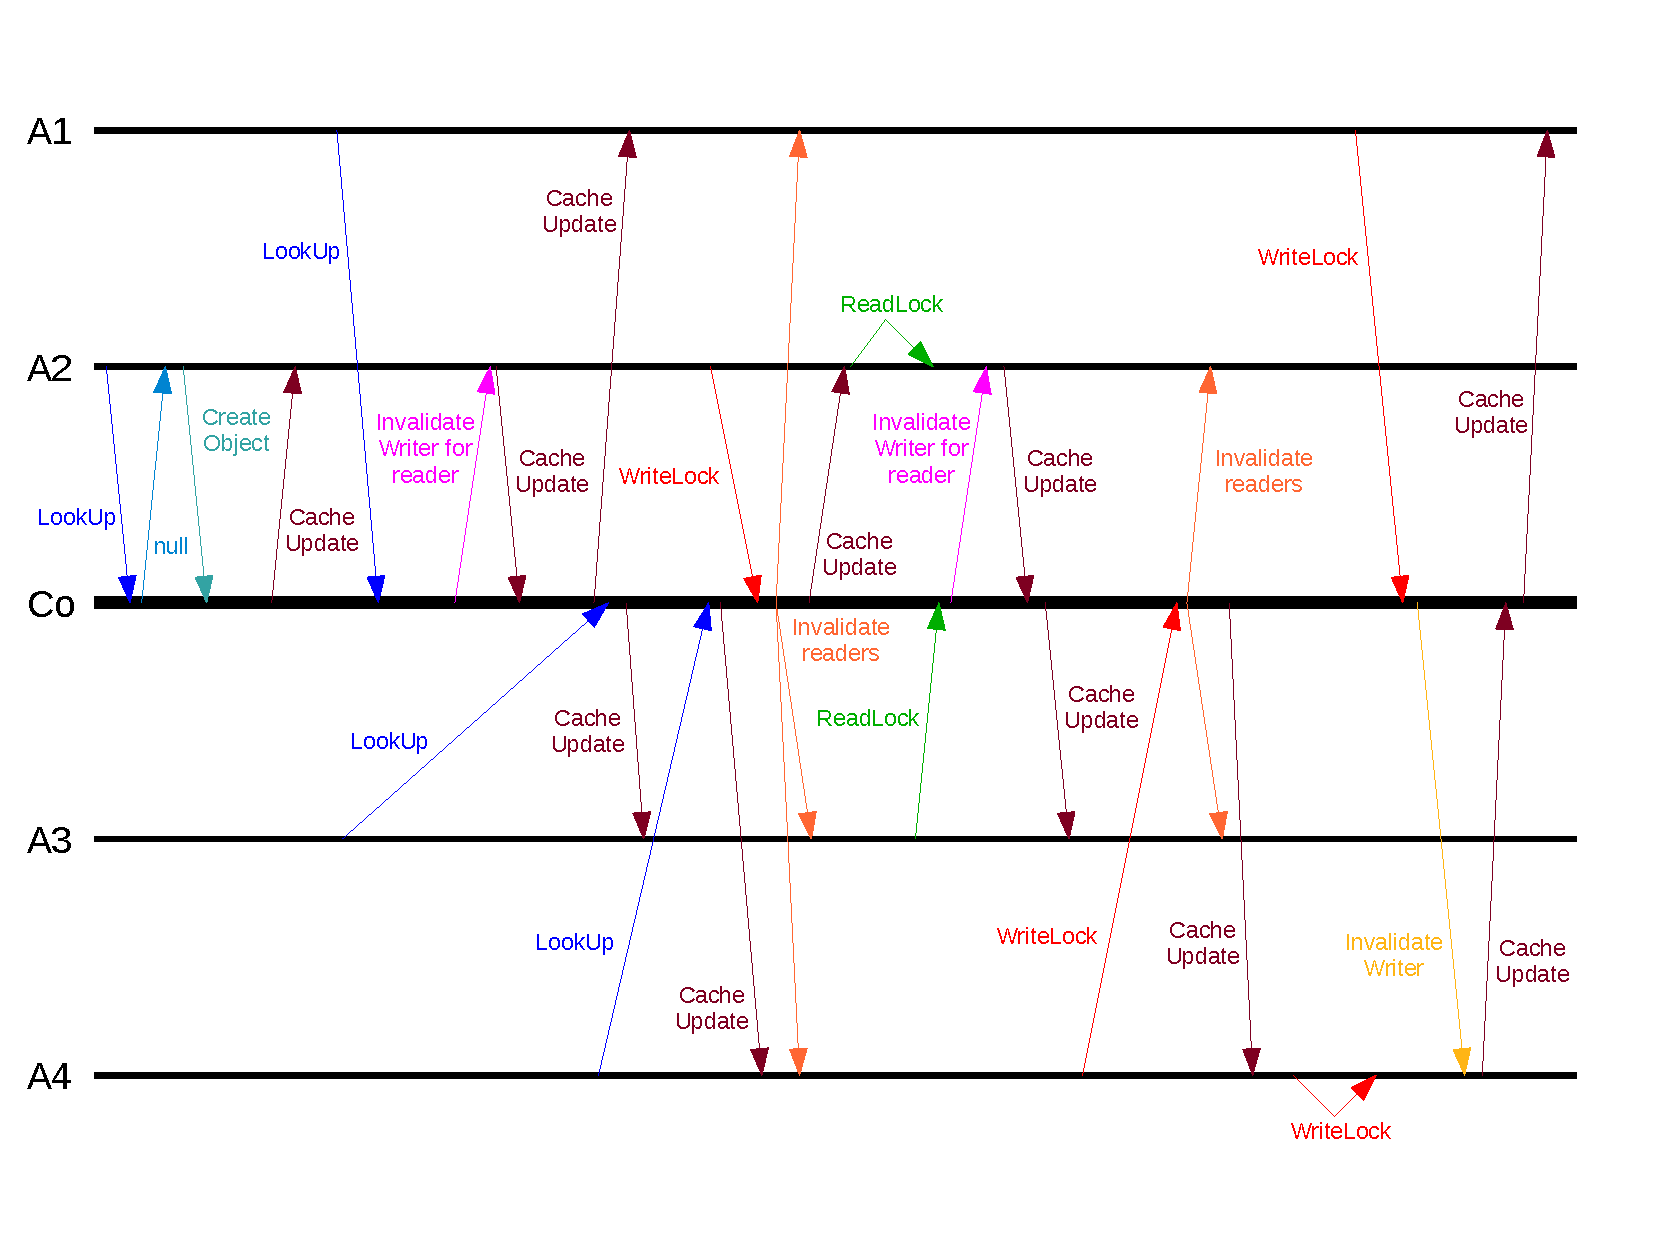
\includegraphics[width=16.85cm, clip, trim=0.4cm 1.5cm 0.6cm 2cm]{sch1}
\end{center}

\hrule\hrule \vspace{5mm}
\begin{huge}Additional features
\end{huge}
\vspace{5mm} \hrule\hrule

\section{Transaction}

The JAVANAISE librairy includes a basic transaction system. The purpose is to be able to realize multiple call of the functions of the object without any modification coming from the other servers. Four functions can be called for each object :

\begin{itemize}
\item \texttt{start()} $\rightarrow$ This function starts the transaction. After the call to \texttt{start()}, the updated state of the object will not be sent to the coordinator until the end of the transaction. 
\item \texttt{commit()} $\rightarrow$ This function validates the transaction. The current state of the object is sent to the coordinator.
\item \texttt{rollback()} $\rightarrow$ This function cancels the transaction. The current state is forgotten and replaced by the state known by the coordinator.
\item \texttt{rollbackToMe()} $\rightarrow$ This function cancels the transaction. The current state is forgotten and replaced by the state saved at the moment of the call to \texttt{start()}. This state is also sent to the coordinator.
\end{itemize}

\begin{center}
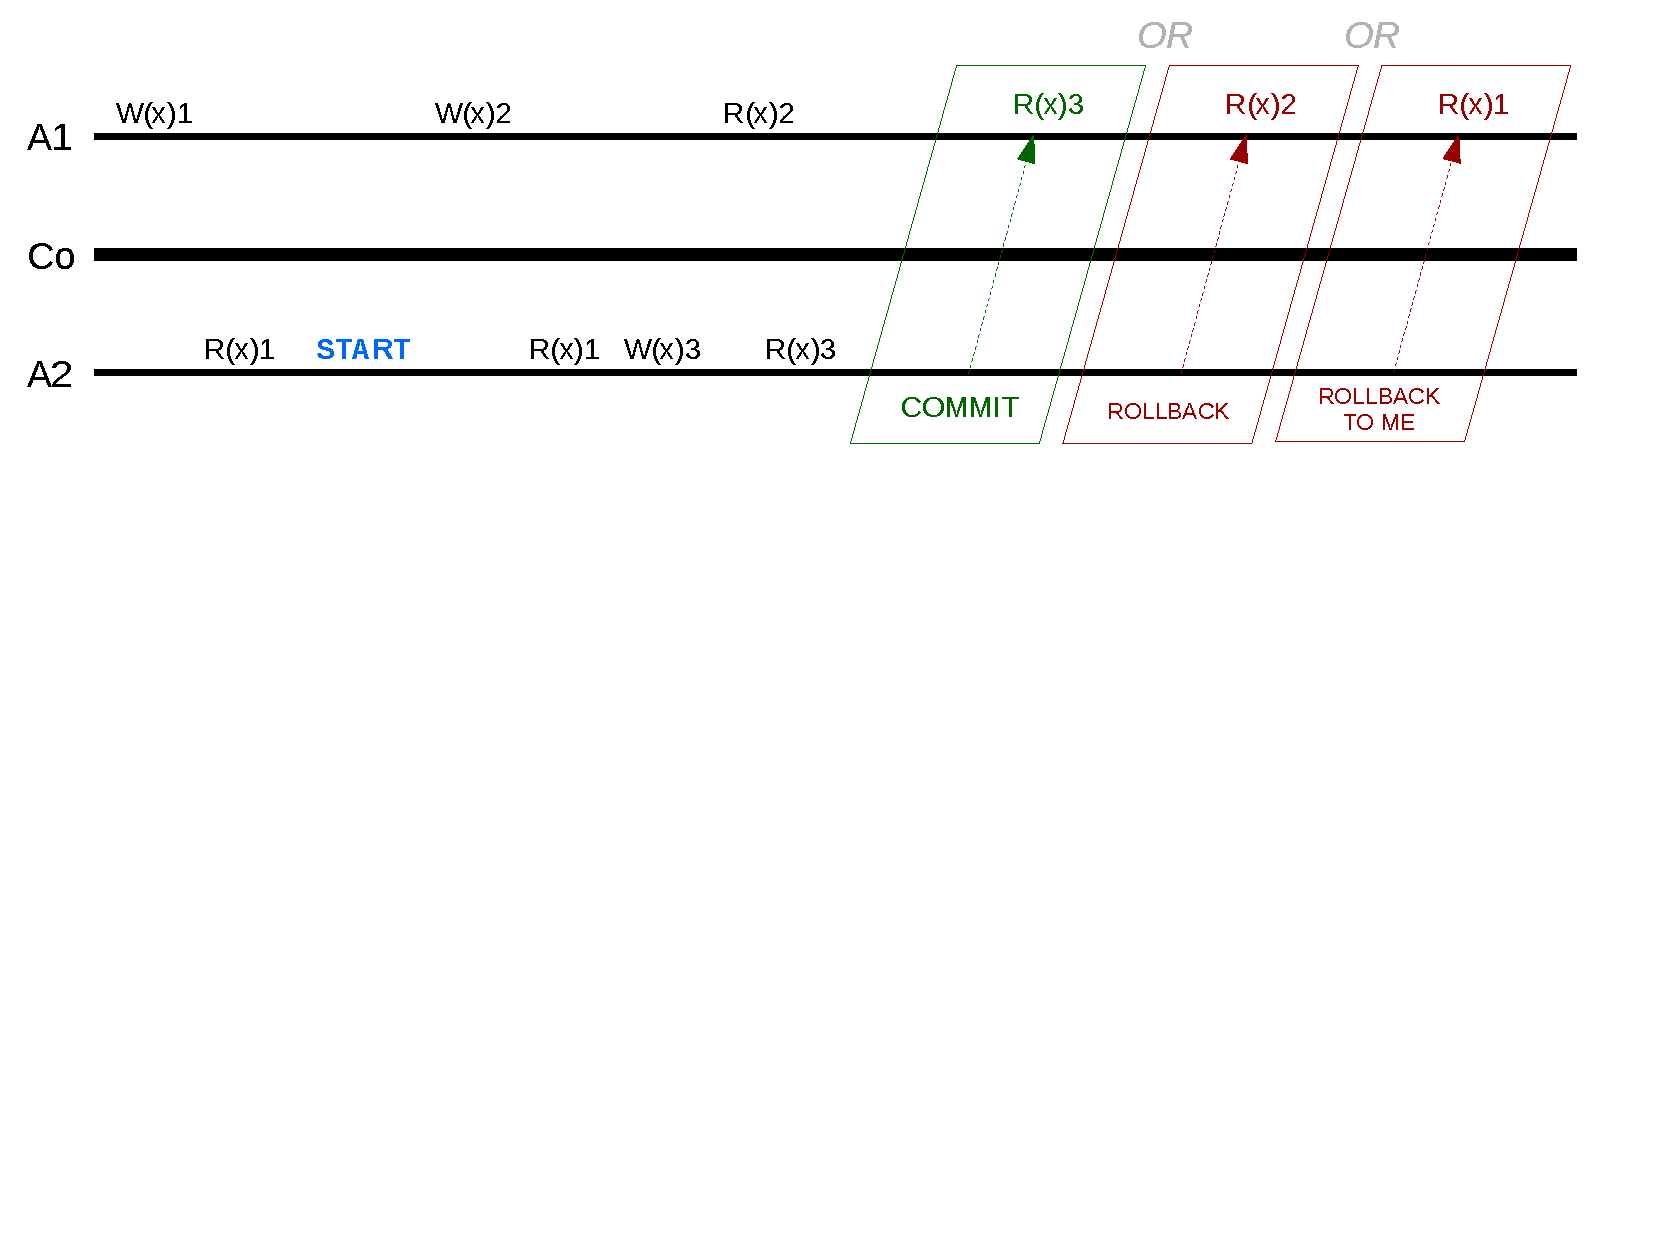
\includegraphics[width=16.85cm, clip, trim=0.4cm 13.2cm 0.6cm 0.2cm]{sch2}
\end{center}

\section{Coordinator breakdown handling}

\subsection{No coordinator available at launch}

If the application can't get the coordinator when starting, a mechanism of wait is set up. Every 5 seconds, the application test again if the coordinator is reachable. The execution of the application starts again normally when the test is successfull.

\subsection{Breakdown of the coordinator during execution}

At any moment of the execution, if the application can't reach the coordinator, the message \textit{"Breakdown of the coordinator"} is shown and the application starts to wait the coordinator. A notification is sent to the application when the coordinator is restart and the execution of the application starts again normally. \\
\vspace{-0.5cm}
\begin{table}[h]
    \begin{center}
    \begin{tabular}{ >{\centering\arraybackslash}m{0.1in} >{\arraybackslash}m{5.8in} }
    \vspace{-0.8mm} \danger & The coordinator needs to be restart with \texttt{start(TRUE)}. \\
    \vspace{-0.8mm} \danger & The updated state of an object can be lost because of a breakdown.
  \end{tabular}
  \end{center}
\end{table}



\end{document}
